% Terms and Definitions
%TODO maybe move stuff from chapter 1 in this chapter
\chapter{Metrics and Measurement Methods}

[tbd]

\begin{itemize}
	\item Last chapter...
	\item This chapter: In this chapter, I will cover measurement methods and discuss common performance metrics.
	\begin{itemize}
		\item This chapter should cover all relevant terms and definitions within web performance measurement
		\item How terms can be structured / taxonomy
		\item Ambiguity of definitions
	\end{itemize}
	\item In the next chapter...
\end{itemize}


- Technical Background:
	- Network
	- Front End: Navigation and CRP
	
- Metrics

- Measuring Methods



% TODO
% IF possible use more cool tables


% ---------------------------------------------------------------------------------------------------
% ---------------------------------------------------------------------------------------------------


%TODO find better title
\section{Technical Background}

% [Introduction]
- Brief technical introduction
- It is important to understand how things work, because Metrics and also how to measure them are derived from those processes


% [3 Entities: FE, BE, Network]
In his code talk 2016, Witt identifies three main areas or bottlenecks where bad performance is being produced: In the Frontend, the Backend, and on the network layer.  % cite 2016 Witt or just say this ??
The Front End is everyhting the user sees on the screen, client, UI, browser, sends requests to a back end, etc.
The Back End is the logic, servier, also data base, handles requests and sends responses to a front end
Network is what connects clients and servers, FE and BE, infrastructure element composed of routers, cables, wireless connections etc.


- BE is not discussed (server time, data base, etc.)
- Section X is about Network
- Section X is about Front end: how browser works, crp, 
- How to optimise websites is not part of this thesis



% --------------------------------------------------------------------------------------------
% --------------------------------------------------------------------------------------------


\subsection{Network Questions}

\subsubsection{Latency vs Bandwidth}

There are two important attributes when discussing network performance: Latency and Bandwidth.
- Key takeaway: Latency is bottleneck

% 2013 Grigorik
- Very nice graphic...
- Ch 10: Why ? The previous results are a surprise to many, but they really should not be, as they are a direct consequence of the performance characteristics of the underlying protocols: TCP handshakes, flow and congestion control, and head-of-line blocking due to packet loss. Most of the HTTP data flows consist of small, bursty data transfers, whereas TCP is optimized for long-lived connections and bulk data transfers.


% [Bandwidth]

% 2013 Grigorik
Chapter 1 :
- Bandwidth: Maximum throughput of a logical or physical communication path
- Bandwidth can more easily be increased with more cables and WDM upgrades

Chapter 10:
- Bandwidth: For video


% [Latency]

% 2013 Grigorik
Chapter 1 :
- Latency: The time from the source sending a packet to the destination receiving it
- Decrease latency is not that simple due to physical restrictions. Data already travels with 2/3 speed of light
- Use other techniques such as CDNs, caching, pre-fetching, etc
- CDN: Help against this issue. Put stuff close to client

Chapter 10:
- when it comes to everyday web browsing, which requires fetching hundreds of relatively small resources from dozens of different hosts, roundtrip latency is the limiting factor
- Latency as a Performance Bottleneck
-  wireless latencies are significantly higher, making networking optimization a critical priority for the mobile web.


% Grigorik Conference Talk https://www.youtube.com/watch?v=PkOBnYxqj3k&ab_channel=IlyaGrigorik
% And slides https://www.igvita.com/slides/2013/fluent-perfcourse.pdf
- Why are mobile latencies so high?
- Why is latency the bottleneck?


% How Browsers Work https://developer.mozilla.org/en-US/docs/Web/Performance/How_browsers_work
- Latency as main threat
- "Network latency is the time it takes to transmit bytes over-the-air to computers"


% Understanding Latency https://developer.mozilla.org/en-US/docs/Web/Performance/Understanding_latency
- time it takes for a packet of data to travel from source to a destination

What is Latency?:
- amount of time it takes from when a request is made by the user to the time it takes for the response to get back to that user
- For first request latency is longer as it includes a DNS lookup, a TCP handshake, the secure TLS negotiation
- Latency describes the amount of delay on a network or Internet connection
- One of the main aims of improving performance is to reduce latency.
- We can determine the amount of latency by measuring the speed with which the data moves from one network location to another.
- Latency can be measured one way or entire round-trip
- Generally measured in round-trip


% [Conclusion]

% 2016 Witt code talks
- latency impact: 2 times bandwith makes no difference, half of latency makes half of load time

- For more details on networking like TCP TLS etc always cf to Grigorik

% Some direct implications for performance measurement ?
% Understanding Latency https://developer.mozilla.org/en-US/docs/Web/Performance/Understanding_latency
Network throttling:
- Emulate download speed, upload speed, and minimum latency

% 2014 Hogan https://designingforperformance.com/
Chapter 2 The Basics of Page Speed
% "Steve Souders says, “80 to 90% of the end user response time is spent on the frontend.” --> Find and cite this
- use this as transition to Front End Section



\subsubsection{Navigation Process}

- I will explain briefly the general navigation process
- Last part of this process is when browser receives finally the HTML / Document. 
- This section briefly describes the steps from start to end.
- On the network, establishing a connection with DNS etc.
- Then the server creates the response, maybe calls a DB etc.
- What then happens in the browser is part of the next section.
- What happens then is explained in CRP

- Process From Start when user types in URL and hits enter, until the end when he sees the website fully loaded on his screen

% [This famous image]
% https://www.w3.org/TR/navigation-timing/

\begin{figure}[h!]
\begin{center}
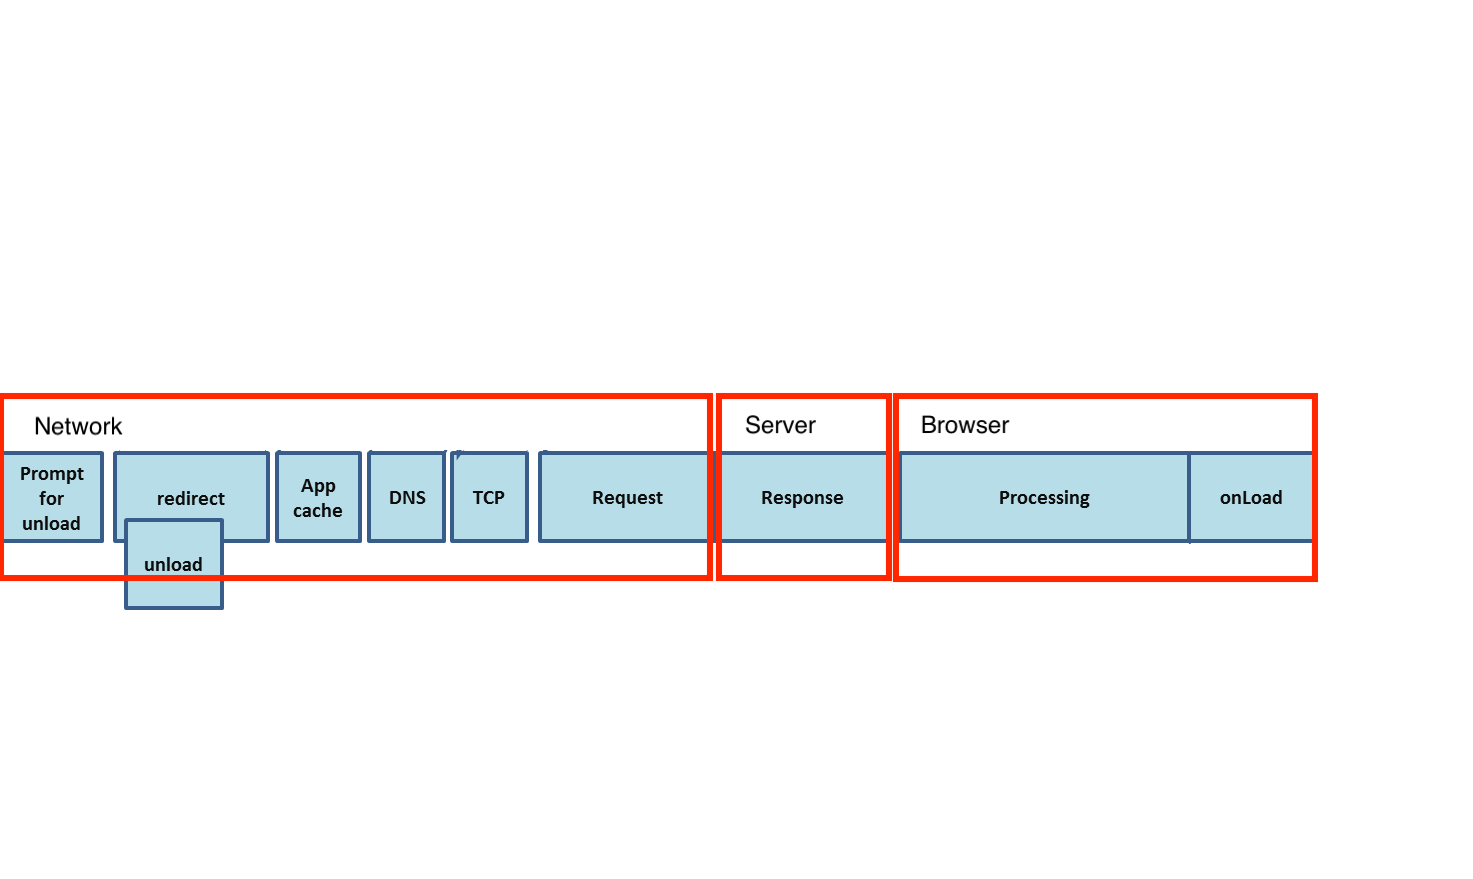
\includegraphics[width=0.8\textwidth]{timing_overview.png}
\caption{Timing Overview}
\label{img:timing_overview}
\end{center}
\end{figure}


% 2014 Hogan https://designingforperformance.com/
Chapter 2 The Basics of Page Speed
How Browsers Render Content:
- Steps between user types and submits URL and sees page on screen



% ----------------------------------


% [DNS]

% How Browsers Work https://developer.mozilla.org/en-US/docs/Web/Performance/How_browsers_work
DNS Lookup:
- translate URL to IP address. Can be cached by browser
- Must be done for each unique URL, e.g. when images are from different server

% 2014 Hogan https://designingforperformance.com/
Chapter 2 The Basics of Page Speed - How Browsers Render Content:
- DNS Lookup (only when unknown domain)

% 2016 Witt code talks
Network:
- DNS lookup

% Understanding Latency https://developer.mozilla.org/en-US/docs/Web/Performance/Understanding_latency
Network Timings:
- DNS resolution: Time it took for DNS lookup



% ----------------------------------


% [TCP]

% How Browsers Work https://developer.mozilla.org/en-US/docs/Web/Performance/How_browsers_work
TCP Handshake:
- 3-way-handshake between client and server
-> 3 more requests between client and server
TCP Slow Start / 14kb rule:
- Is an algorithm: Slow start gradually increases the amount of data transmitted until the network's maximum bandwidth can be determined
- Avoid congestion
- This is not part of TCP handshake but for first HTTP request
- Initial response is 14Kb, second one is 28, etc.
- Congestion Control algorithms: determine send rate

% 2014 Hogan https://designingforperformance.com/
Chapter 2 The Basics of Page Speed - How Browsers Render Content:
- Connections:
- Number of connections is not the same as number of requests it takes to load the page
- SSL Negotiation explained
- Persistent Connection: Browser keeps connection open for multiple requests
- Parellell possible open connections, 6 for Chrome
- To each domain one connection ??
- TTFB


% ----------------------------------


% [TLS]

% How Browsers Work https://developer.mozilla.org/en-US/docs/Web/Performance/How_browsers_work
TLS Negotiation:
- Make connection secure by changing cipher etc
-> 3 more round trips

-> At this point already 8 round trips

% 2016 Witt code talks
Network:
- Initial connection: TCP Handshake and TLS handshake
- time to first byte: When first page data byte receives on client side
- content download
-> Max 6 parallel connections


% Understanding Latency https://developer.mozilla.org/en-US/docs/Web/Performance/Understanding_latency
Network Timings:
- Blocked: When a request is in queue
- Blocking happens when there are too many simultaneous connections to single server over HTTP

% Understanding Latency https://developer.mozilla.org/en-US/docs/Web/Performance/Understanding_latency
- TCP, TLS
- Sending, Waiting, Receiving



% ----------------------------------



% [HTTP Request and Response]

% How Browsers Work https://developer.mozilla.org/en-US/docs/Web/Performance/How_browsers_work
Request/Response:
- HTTP Get request by client to server
- Response contains first byte of data received -> Time to First Byte Metric! -> link here to metric description


% 2016 Witt code talks
- Avg total requests % https://httparchive.org/



% ----------------------------------


% [Rendering/Parsing: Transition to CRP]

- Navigation now finished
- From this derived are Navigation Timings and Resource Timings -> See chapter X metrics 

- What happens exactly when the browser received the first data?
- CRP enters the stage see section X


% ----------------------------------

% [Optimization and Performance]
%TODO maybe move each optimization trick to his corresponding section ?

% How Browsers Work https://developer.mozilla.org/en-US/docs/Web/Performance/How_browsers_work
- Goal: minimize the amount of time a navigation takes to complete


% Grigorik Conference Talk https://www.youtube.com/watch?v=PkOBnYxqj3k&ab_channel=IlyaGrigorik
% And slides https://www.igvita.com/slides/2013/fluent-perfcourse.pdf
- Optimize your networking stack!



% 2014 Hogan https://designingforperformance.com/
Chapter 2 The Basics of Page Speed - How Browsers Render Content:
- Browsers try to parallelize requests for content
- Requests: Optimizing size and amount of requests has big impact on performance, e.g. get all images in one requests using Sprites

Page Weight is somewhat important:
- Sum of all file sizes
- Averages in httparchive, which i also used in one approach % https://httparchive.org/reports/state-of-the-web?start=latest

Other Impacts on Page Speed
- "environmental factors"
- Geography, CDNs
- Network
- Browser


% 2016 Witt code talks
- Possible Improvements:
- HTTP2
- Avoid redirects
- Caching headers
- CDNs
- Single Page Apps





% --------------------------------------------------------------------------------------------
% --------------------------------------------------------------------------------------------



\subsection{Front End: Critical Rendering Path}

- This section explains what happens on the Front End, that is in the browser

- Critical Rendering Path: How the Browser works, what exactly happens with the received html etc.
- How Browser works, CRP: First byte, style, layout etc.
- External Resources


The CRP is the last part of the whole process.
In happens in the browser once it received the data / document / HTML

There are a sequence of steps the browser goes through to render the page.

Basic idea:  Convert HTML, CSS and JS to actual pixels on the screen


% How Browsers Work https://developer.mozilla.org/en-US/docs/Web/Performance/How_browsers_work
Parsing:
- Starts when browser received fist data
- HTML, CSS, and JavaScript have to be parsed.
- Parsing is the step the browser takes to turn the data it receives over the network into the DOM and CSSOM, which is used by the renderer to paint a page to the screen.




% [Single Thread]

% How Browsers Work https://developer.mozilla.org/en-US/docs/Web/Performance/How_browsers_work
- This is somewhat the bottleneck or the technical state of the browser
- Browser is single threaded
- Still: Enable smooth interaction: scrolling, responsive to touch, etc.
- Render time is key
- Goal: Main thread can complete all the work and still is available to handle user interaction
-> Improvement: Understand single thread concept of browser and minimize main threads responsibilities
-> Should lead to: rendering is fast and smooth and responses to interactions are immediate



% [CRP Steps]

The CRP consists of multiple steps.
Once the HTML is received, the browser will parse it to the DOM.
The HTML references CSS and JS files.

CSS will be parsed to CSSOM.

JS needs also to be executed.

Render Tree: Once DOM and CSSOM are available, the Render Tree is being created.

Layout: When the Render Tree is available, Layout is happening.

Paint: Finally, pixels can be printed on the screen.

\begin{figure}[h!]
\begin{center}
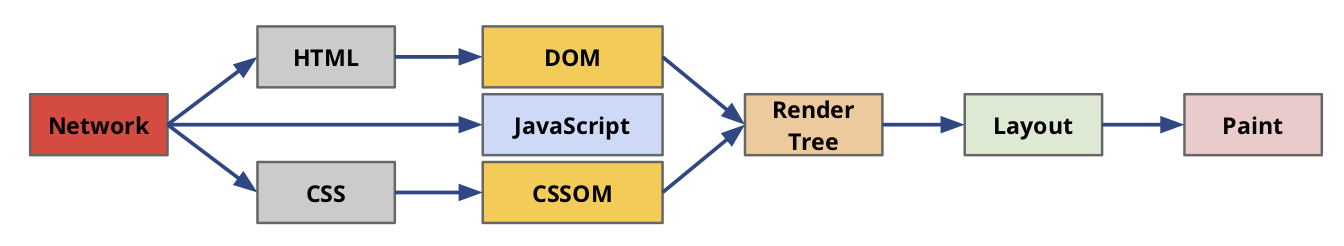
\includegraphics[width=0.7\textwidth]{crp.png}
\caption{Critical Rendering Path}
\label{img:crp}
\end{center}
\end{figure}

The individual steps are discussed below.




% ------------------------------------------------------------

\paragraph{From HTML to DOM}


% [DOM]


- DOM:
	- Converting HTML to DOM:
		- Defined in HTML specification
		- Characters -> Tokens -> Nodes -> DOM

	- Tokenizer:
		- <html><head><meta name="viewport">
		-> Tokens: [StartTag: HTML], [StartTag: head], [Tag: meta], [EndTag: head], ...

	- Convert tokens to node objects:
		-> DOM:
			- Tree structure
			- Objects also contain properties

		- Created incrementally
		-> Beneficial for performance
		- Return partial HTML


% https://developers.google.com/web/fundamentals/performance/critical-rendering-path/constructing-the-object-model
- Bytes -> characters -> tokens -> nodes -> object model.
- HTML markup is transformed into a Document Object Model (DOM)
- The DOM tree captures the properties and relationships of the document markup, but it doesn't tell us how the element will look when rendered. That’s the responsibility of the CSSOM.

% https://developer.mozilla.org/en-US/docs/Web/Performance/Critical_rendering_path
- DOM


% https://medium.com/@luisvieira_gmr/understanding-the-critical-rendering-path-rendering-pages-in-1-second-735c6e45b47a
- DOM




% How Browsers Work https://developer.mozilla.org/en-US/docs/Web/Performance/How_browsers_work
- DOM: internal representation of the markup for the browser
- DOM is also exposed, and can be manipulated through various APIs in JavaScript
- Browser will begin parsing as soon as data received: Important to include most important stuff in first 14Kb

1. Building the DOM tree:
- Build DOM tree by processing HTML markup (tokenization, tree construction)
- Browser requests non-blocking resources and continues parsing
- CSS does not block parsing
- scripts which are not async or defer block parsing -> excessive scripts can be a significant bottleneck

Optimisation: Preload scanner:
- This process occupies main thread while browser is building DOM Tree
- parse through the content available and request high priority resources like CSS, JavaScript, and web fonts.
- will retrieve resources in the background so that by the time the main HTML parser reaches requested assets, they may possibly already be in flight, or have been downloaded
- CSS fetch does not block HTML parsing but JS



% https://medium.com/jspoint/how-the-browser-renders-a-web-page-dom-cssom-and-rendering-df10531c9969
As we have learned that DOM tree generation is incremental which means as the browser reads HTML, it will add DOM elements to the DOM tree


% 2014 Hogan https://designingforperformance.com/
Chapter 2
- CRP:
- Creation of DOM Tree out of HTML



% ------------------------------------------------------------

\paragraph{From CSS to CSSOM}


% [CSSOM]

- DOM and CSSOM are independent data structures.

- CSSOM:
	- Characters -> Tokens -> Nodes -> CSSOM
	- Cascading rules / style sheet: Children inherit styling rules of parent
	- CSS rules cascade down
	- Partial CSS Tree not possible, because rules can be overwritten
	- Browser blocks page rendering until it receives all of the CSS
	-> CSS is render blocking

	- More specific rules are more expensive
	
	
- CSS Blocking Operation:
	- CSS blocks rendering:
	-> Rules can be overwritten, so that content can't be rendered until CSSOM is complete
	- <link rel="stylesheet" href="a.css">: Browser waits on this line, until file is received
	- Better to add styles in single file

	- JS can change styling of page -> Browser blocks JS until CSS is resolved
	
	
% https://developers.google.com/web/fundamentals/performance/critical-rendering-path/render-blocking-css



% https://developers.google.com/web/fundamentals/performance/critical-rendering-path/constructing-the-object-model
- CSS Stylesheet
- The CSS bytes are converted into characters, then tokens, then nodes, and finally they are linked into a tree structure known as the "CSS Object Model" (CSSOM):


% https://developer.mozilla.org/en-US/docs/Web/Performance/Critical_rendering_path
- CSSOM

% https://medium.com/@luisvieira_gmr/understanding-the-critical-rendering-path-rendering-pages-in-1-second-735c6e45b47a
- CSSOM



% https://medium.com/jspoint/how-the-browser-renders-a-web-page-dom-cssom-and-rendering-df10531c9969
- Render blocking CSS
- Unlike the DOM tree, CSSOM tree construction is not incremental and must happen in a specific manner.
- browsers can’t build the CSSOM tree incrementally as it reads the CSS content. The reason for that is, a CSS rule at the end of the file might override a CSS rule written at the top of the file
- CSS is a render-blocking resource
- Once the browser makes a request to fetch an external stylesheet, the Render Tree construction is halted.




% 2014 Hogan https://designingforperformance.com/
Chapter 2
- Request for stylesheet will block parsing -> CSS is render-blocking resource
- Creation of CSSOM


% How Browsers Work https://developer.mozilla.org/en-US/docs/Web/Performance/How_browsers_work
2. Building the CSSOM:
- Process CSS and build CSSOM tree
- Similar to DOM
- Usually very fast





% ------------------------------------------------------------

\paragraph{What happens with JavaScript}


% [JavaScript]


- JS Blocking Operation:
	- <script src=""></script>: Will be executed directly when received
	- Do i need to run JS before DOM is created?
	-> Add at end of <body>

- Async:
	- <script src="" async></script>
	- Loads script asynchronously to the page
	- DOM parsing continues
	
	
% How Browsers Work https://developer.mozilla.org/en-US/docs/Web/Performance/How_browsers_work
- scripts which are not async or defer block parsing -> excessive scripts can be a significant bottleneck



% How Browsers Work https://developer.mozilla.org/en-US/docs/Web/Performance/How_browsers_work
Other Processes:
- JavaScript Compilation: JavaScript is interpreted, compiled, parsed and executed.



% https://developers.google.com/web/fundamentals/performance/critical-rendering-path/adding-interactivity-with-javascript


% https://medium.com/jspoint/how-the-browser-renders-a-web-page-dom-cssom-and-rendering-df10531c9969
- Parser blocking JS
- Internal: script elements are parser-blocking. Every external file requests such as image, stylesheet, pdf, video, etc. do not block DOM construction (parsing) except script (.js) file requests.
- When the browser encounters a script element, if it an embedded script, then it will execute that script first and then continue parsing the HTML to construct the DOM tree. So all embedded scripts are parser-blocking

- External:
- If the script element is an external script file, the browser will start the download of the external script file off the main thread but it will halt the execution of the main thread until that file is downloaded. That means no more DOM parsing until the script file is downloaded
- Once the script file is downloaded, the browser will first execute the downloaded script file on the main thread (obviously) and then continue with the DOM parsing. If the browser again finds another script element in HTML, it will perform the same operation

- async:
When DOM parser encounters an external script element with async attribute, it will not halt the parsing process while the script file is being downloaded in the background. But once the file is downloaded, the parsing will halt and the script (code) will be executed.


- defer:
We also have a magical defer attribute for the script element which works similar to the async attribute but unlike the async attribute, the script doesn’t execute even when the file is fully downloaded. All defer scripts are executed once the parser has parsed all HTML which means the DOM tree is fully constructed. Unlike async scripts, all defer scripts are executed in the order they appear in the HTML document (or DOM tree).


All normal scripts (embedded or external) are parser-blocking as they halt the construction of DOM. All async scripts (AKA asynchronous scripts) do not block parser until they are downloaded. As soon as an async script is downloaded, it becomes parser-blocking. However, all defer scripts (AKA deferred scripts) are non-parser-blocking script as they do not block the parser and execute after the DOM tree is fully constructed.




% 2014 Hogan https://designingforperformance.com/
Chapter 2
- JS blocks DOM construction unsless its declared async or defer





% ------------------------------------------------------------


\paragraph{Building the Render Tree}

% [Render Tree]


- Render Tree:
	- DOM + CSSOM: Content and styles
	- Only captures visible content
	- Display: none -> Children also skipped, because style cascades down
	
	
% https://developers.google.com/web/fundamentals/performance/critical-rendering-path/render-tree-construction
- The DOM and CSSOM trees are combined to form the render tree.
- Render tree contains only the nodes required to render the page.
- Layout computes the exact position and size of each object.
- The last step is paint, which takes in the final render tree and renders the pixels to the screen.


% How Browsers Work https://developer.mozilla.org/en-US/docs/Web/Performance/How_browsers_work
Render:
- Build Render Tree
- Create render tree out of DOM and CSSOM


% https://developer.mozilla.org/en-US/docs/Web/Performance/Critical_rendering_path
- Render Tree


% https://medium.com/@luisvieira_gmr/understanding-the-critical-rendering-path-rendering-pages-in-1-second-735c6e45b47a
- Render Tree




% Grigorik Conference Talk https://www.youtube.com/watch?v=PkOBnYxqj3k&ab_channel=IlyaGrigorik
% And slides https://www.igvita.com/slides/2013/fluent-perfcourse.pdf
- CRP:
- Render Tree: With DOM and CSSOM



% 2014 Hogan https://designingforperformance.com/
Chapter 2
- Creation of Render Tree by combining DOM and CSSOM
- Start Render Metric




% ------------------------------------------------------------

\paragraph{Layout}




% [Layout]

- Layout:
	- Position of the elements on the page
	- Calculating positions and dimensions
	- Layout viewport size
	- <meta name="viewport" content="width=device-width">
	- Default width: 980px, used when meta tag is not set

	- Layout triggered by device orientation, window resize, adding or removing from DOM tree, etc.
	

% How Browsers Work https://developer.mozilla.org/en-US/docs/Web/Performance/How_browsers_work
4. Layout:
- Run layout on render tree
- Compute geometry of each node
- Exact size and location of each object
- Subsequent changes are called reflow, e.g. when image is received later without specify its size


% https://developer.mozilla.org/en-US/docs/Web/Performance/Critical_rendering_path
- Layout


% https://medium.com/@luisvieira_gmr/understanding-the-critical-rendering-path-rendering-pages-in-1-second-735c6e45b47a
- Layout


% Grigorik Conference Talk https://www.youtube.com/watch?v=PkOBnYxqj3k&ab_channel=IlyaGrigorik
% And slides https://www.igvita.com/slides/2013/fluent-perfcourse.pdf
- Layout



% https://developers.google.com/web/fundamentals/performance/critical-rendering-path/render-tree-construction




% ------------------------------------------------------------

\paragraph{Paint}


% [Paint]


% How Browsers Work https://developer.mozilla.org/en-US/docs/Web/Performance/How_browsers_work
5. Paint:
- Paint nodes on screen
-> First Meaningful Paint
- Time to Interactive


% https://developer.mozilla.org/en-US/docs/Web/Performance/Critical_rendering_path
- Paint



% https://medium.com/@luisvieira_gmr/understanding-the-critical-rendering-path-rendering-pages-in-1-second-735c6e45b47a
- Paint


% Grigorik Conference Talk https://www.youtube.com/watch?v=PkOBnYxqj3k&ab_channel=IlyaGrigorik
% And slides https://www.igvita.com/slides/2013/fluent-perfcourse.pdf
- Paint


% https://developers.google.com/web/fundamentals/performance/critical-rendering-path/render-tree-construction




% ------------------------------------------------------------


\paragraph{What else?}

Additional infos here



% [Compositing ?]




% [Conclusion, Optimizations]

% 2013 Grigorik
Chapter 10:
- Script execution can issue a synchronous doc.write and block DOM parsing and construction
- JavaScript can also block on CSS
- DOM construction cannot proceed until JavaScript is executed, and JavaScript execution cannot proceed until CSSOM is available
-> styles at the top, scripts at the bottom best practice
- Different browsers implement different logic for when, and in which order, the individual resource requests are dispatched. As a result, the performance of the application will vary from browser to browser.


% Grigorik Conference Talk https://www.youtube.com/watch?v=PkOBnYxqj3k&ab_channel=IlyaGrigorik
% And slides https://www.igvita.com/slides/2013/fluent-perfcourse.pdf
- Optimize the critical rendering path!


% 2014 Hogan https://designingforperformance.com/
- Optimizations of CRP:
- media types and queries on css resources, which makes them non-blocking
- Load JS efficient
- Priotize requests for above the fold
- etc. % Do i need to explain this ??

Chapter 4:

CSS and JavaScript Loading:
- Rules:
- Load CSS in head
- CSS blocks rendering

- Load JS at bottom of the page
- Load Async
- JS blocks DOM construction, because browser knows that content from script tag may change Render Tree
- async tag will execute script once its ready, but order is not berücksichtigt
- Anything that loads late and changes UI can cause layout shifts
- 3rd party scripts: Need additional DNS lookup, should not be single point of failure


% https://developer.mozilla.org/en-US/docs/Web/Performance/Critical_rendering_path
- Optimizing for CRP


% https://medium.com/@luisvieira_gmr/understanding-the-critical-rendering-path-rendering-pages-in-1-second-735c6e45b47a
- Optimizing


% Grigorik Conference Talk https://www.youtube.com/watch?v=PkOBnYxqj3k&ab_channel=IlyaGrigorik
% And slides https://www.igvita.com/slides/2013/fluent-perfcourse.pdf
-  HTML is parsed incrementally
- Rendering is blocked on CSS...
- Optimize the critical rendering path!

- DOM construction can't proceed until JavaScript is fetched
- DOM construction can't proceed until JavaScript is executed
- Sync script will block the DOM + rendering of your page:

- Async all the things! nice image about async attribute


- Optimizing DOM:
	- Minify HTML
	- Compression
	- Cache in Browser


- Unblocking CSS:
	- Media queries: for responsive design
	-> Move media queries to separate file
	- <link rel="stylesheet" href="style-print.css" media="print">
	-> Will not block rendering


- Optimizing JS:
	- Minify, compress, cache
	- JS is parser blocking
	- Script tag blocks DOM construction
	- For external JS, browser waits until JS is fetched and executed
	- CSS blocks rendering and JS execution

	- Load and execute script after page is loaded
	- Page is loaded: Browser fires onload event
	- Async attribute:
		- <script src="a.js" async></script>
		- Does not block CRP (DOM construction, CSSOM)

	- async attribute not applicable on inline scripts
	- Inline script blocks CSSOM unless included before CSS request


- General Strategies:
	- Minify, compress, cache (HTML, CSS, JS)

	- Minimize use of render blocking resources (CSS):
		- Media queries
		- Inline CSS

	- Minimize use of parser blocking resources (JS):
		- Defer JS execution
		- async attribute


	-> Minimize Bytes
	-> Reduce critical resources
	-> Shorten CRP length

















% https://developers.google.com/web/fundamentals/performance/critical-rendering-path/analyzing-crp




% --------------------------------------------------------------------------------------------






\subsection{Conclusion Technical Background}

% Connection to Optimisation

% We could see that performance Metrics are directly derived from this process

% Metrics will be discussed next

% After that, i will talk about how to actually measure the metrics



% 2013 Grigorik
- Browser optimizations...

% 2016 Witt code talks
- tools available:
- Profiling: GTMetrix, WebPageTest, PageSpeed Insigths
- Inlining and Optimization: Critical, PostCSS, processhtml
- Minification and Compression: Goole Closure, tinyPng, Uglifycss and cssmin



%TODO add this ??
% [JavaScript Parsing]
% https://medium.com/reloading/javascript-start-up-performance-69200f43b201






% ---------------------------------------------------------------------------------------------------------------------------------------
% ---------------------------------------------------------------------------------------------------------------------------------------




\section{Measurement Methods}


% [Introduction]
- synthetic monitoring
- RUM
- other methods briefly described


\begin{itemize}
\item Explanation and comparison of synthetic and real-user monitoring with concrete examples
\item Short overview of other measuring methods such as log analysis or surveys
\end{itemize}



% About measuring web performance
% Why web performance? As we saw its important for business





% https://developer.mozilla.org/en-US/docs/Web/Performance/Rum-vs-Synthetic
synthetic:
- lab environment: geography, network, device, browser, etc.
- control variables to identify performance issues. this does not reflect real world and real user experience
- automated
- simulate user paths
- traffic is generated artificial and is not by real users
 - can also be used for live system monitoring
 - fairly easy to implement, inexpensive

RUM:
- measure from real users machine
- part of page tagging (same technique with including some JS)
- measures actual use cases



% 2013 Grigorik https://hpbn.co/primer-on-web-performance/
- Synthetic and Real-User Performance Measurement



% 2021 Wolle blog post https://medium.baqend.com/mobile-site-speed-measurement-best-practices-ff4a3f91b003
- Log file
- Synthetic: will be discussed in chapter X
- RUM which will be covered in chapter X
- CrUX
- Surveys


% 2016 Kaur: Tools for Measuring the Performance of Websites
- Pingdom
- GTMetrix
- Website Grader
- Site Speed checker




% 2009 Croll


% 2013 Meenan


% 2013 Grigorik




% 2014 Hogan https://designingforperformance.com/
Ch 6 Measuring and Iterating on Performance

- Browser Tools
- Synthetic Testing
- Real User Monitoring
- Changes over Time




% 2015 Cito


% 2016 Viscomi Synthetic Versus RUM


% Eggplant whitepaper




% ----------------------------------------------------------------------------------------------
% ----------------------------------------------------------------------------------------------



\subsection{Synthetic Monitoring}

\begin{itemize}
    \item What is it
    \item How does it work
    \item Application, real life scenario
    \item Examples:
    \begin{itemize}
        \item WebPageTest
        \item Google Lighthouse
        \item Other solutions
    \end{itemize}
\end{itemize}













% ----------------------------------------------------------------------------------------------
% ----------------------------------------------------------------------------------------------



\subsection{Real-User Monitoring}

\begin{itemize}
    \item What is it
    \item How does it work
    \item Application, real life scenario
    \item Examples:
    \begin{itemize}
        \item Google Analyitcs
        \item CrUX
        \item SpeedKit
        \item Other solutions
    \end{itemize}
\end{itemize}

% boomerang Akamai






% ----------------------------------------------------------------------------------------------
% ----------------------------------------------------------------------------------------------



\subsection{Other methods}

Reports such as CruX or http archive
surveys
log files



% 2021 Wolle blog post https://medium.baqend.com/mobile-site-speed-measurement-best-practices-ff4a3f91b003
- Log file
- Synthetic: will be discussed in chapter X
- RUM which will be covered in chapter X
- CrUX
- Surveys




% ---------------------------------------------------------------------------------------------------
% ---------------------------------------------------------------------------------------------------
% ---------------------------------------------------------------------------------------------------
% ---------------------------------------------------------------------------------------------------



\section{Metrics}


% taxonomy ?

% Navigation Events: Exposed by Navigation Timing API: navigationStart, domContentLoaded, etc.
% = Navigation Timings
% Resource Timings ?
%  navigation timing measures the main document's timings whereas the resource timing provides the times for all the assets or resources called in by that main document and the resources' requested resources.




% First list all metrics -> get overview
% Then think about possible categories

% Structure of this chapter ??

% APIs
% Web Vitals and Core Web Vitals

% own / user specific metrics, e.g. time to first tweet for twitter (meenan 2021)


% https://developer.mozilla.org/en-US/docs/Learn/Performance/Perceived_performance




% https://developer.mozilla.org/en-US/docs/Learn/Performance/Measuring_performance
- Compare to competitors
- Compare different versions of your app
- Metrics should be relevant to your users, site, and business goals
- should be collected and measured in a consistent manner
- analyzed in a format that can be consumed and understood by non-technical stakeholders




% ===== START: HERE I WILL LIST ALL METRICS =====

Check out glossary: https://developer.mozilla.org/en-US/docs/Glossary



DNS resolution / DNS lookup time % https://developer.mozilla.org/en-US/docs/Web/Performance/Understanding_latency


Connecting / TCP Handshake time % https://developer.mozilla.org/en-US/docs/Web/Performance/Understanding_latency


TLS Handshake time % https://developer.mozilla.org/en-US/docs/Web/Performance/Understanding_latency


Waiting / Server Response Time ?? % https://developer.mozilla.org/en-US/docs/Web/Performance/Understanding_latency


Receiving / Download Time ?? % https://developer.mozilla.org/en-US/docs/Web/Performance/Understanding_latency




onload Event: % https://developer.mozilla.org/en-US/docs/Web/API/GlobalEventHandlers/onload


DOMContentLoaded Event % https://developer.mozilla.org/en-US/docs/Web/API/Window/DOMContentLoaded_event




Page Load Time: % https://hpbn.co/primer-on-web-performance/
- Has been the de facto metric of the web performance world
- Increasingly insufficient performance benchmark: we are no longer building pages, we are building dynamic and interactive web applications




Start Render % https://designingforperformance.com/basics-of-page-speed/
- tells you how many seconds it took for the browser to begin rendering content


Time to First Byte: % https://developer.mozilla.org/en-US/docs/Glossary/time_to_first_byte

% 2014 Hogan
- First byte that the browser receives
- It’s a good indicator of how quickly the backend of your site is able to process and send back content








First Paint: % https://developer.mozilla.org/en-US/docs/Glossary/First_paint


First Contentful Paint: % https://developer.mozilla.org/en-US/docs/Glossary/First_contentful_paint


First Meaningful Paint: % https://developer.mozilla.org/en-US/docs/Glossary/first_meaningful_paint


Largest Contentful Paint: % https://wicg.github.io/largest-contentful-paint/


Speed Index: % https://developer.mozilla.org/en-US/docs/Glossary/Speed_index


Time to Interactive: % https://developer.mozilla.org/en-US/docs/Glossary/Time_to_interactive






% ===== END: HERE I WILL LIST ALL METRICS =====






% ======== APIs ========

% Measuring Performance https://developer.mozilla.org/en-US/docs/Learn/Performance/Measuring_performance
Performance APIs:
- Many Web APIs available % https://developer.mozilla.org/en-US/docs/Web/API
- Performance API is one API within Web APIs collection: Includes other APIs
- Navigation Timing API: Famous image: Exposes metrics related to navigation events

Tools and metrics:
- 2 categories: Tools for measuring (reporting) and tools for improving
- Reporting:
- PageSpeedInsights
- WebPageTest
- Network:
- Network Panel in DevTools


% https://siusin.github.io/perf-timing-primer/

% https://w3c.github.io/perf-timing-primer/


Performance API % https://developer.mozilla.org/en-US/docs/Web/API/Performance_API
- Includes Performance Timeline API, the Navigation Timing API, the User Timing API, and the Resource Timing API.  ??



Navigation Timing API % https://developer.mozilla.org/en-US/docs/Web/API/Navigation_timing_API
Navigation Timing API Level 2 % https://www.w3.org/TR/navigation-timing-2/

Performance Timeline API % https://developer.mozilla.org/en-US/docs/Web/API/Performance_Timeline

Performance Entry API % https://developer.mozilla.org/en-US/docs/Web/API/PerformanceEntry

PerformanceNavigationTiming % https://developer.mozilla.org/en-US/docs/Web/API/PerformanceNavigationTiming



User Timing API % https://developer.mozilla.org/en-US/docs/Web/API/User_Timing_API

Resource Timing API % https://developer.mozilla.org/en-US/docs/Web/API/Resource_Timing_API



Performance Observer API % https://developer.mozilla.org/en-US/docs/Web/API/PerformanceObserver




%TODO sort this
User Timing API
Navigation Timing API: Level 1 (performance.timing), Level 2 (PerformanceNavigationTiming) ?
Network Information API
Resource Timing API
Paint Timing API
High Resolution Time API
Performance Timeline API
Performance Observer API
Long Tasks API
Element Timing API
Event Timing API
Server Timing API
















\subsection{Introduction}

\begin{itemize}
\item Metrics jungle, difficulty of taxonomy
\item Performance vs UX
\end{itemize}

% 2014 Singal: Types of metrics

% 2015 Bekavac:
% - Metrics for describing visits: entry page, landing page, exit page, visit duration, referrer, ctr
% - Visitors: new visitors, returning visitor, repeat visitor, visits per visitor, recency, frequency
% - Visitor engagement: page exit ratio, bounce rate, page views per visitor
% - Conversion metrics: conversion, conversion rate

% 2019 Enghardt

% 2019 Hussaina:
% Key metrics: visitors, page views, referrers, bounce rate, keywords and phrases






\subsection{"Non-Performance" metrics}
% business related metrics

\begin{itemize}
\item User engagement: session length, bounce rate, etc.
\item Business KPIs: Cart size, conversion rate, etc.
\item QA metadata: Page views, JS errors, etc.
\end{itemize}



% 2004 Peterson
\begin{itemize}
\item Hit
\item Click-Through
\item Page View
\item Visit
\item Visitor / Unique Visitor
\item Referrer
\item Conversion Rate
\item Abandonment Rate
\item Attrition
\item Loyalty, Frequency and Recency
\item Measuring Reach: ...
\item Measuring Acquisition: ...
\item Measuring Conversion: ...
\item Measuring Retention: ...
\end{itemize}


% 2004 Phippen
\begin{itemize}
\item Basic metrics (see table): basic metrics are meaningless
\item Advanced metrics: Customer lifecycle analysis, customer behaviour analysis
\end{itemize}


% 2007 Burby
\begin{itemize}
\item Types: Counts, Rations, KPIs
\item Definitions for all terms, like Page view, unique visitor, etc.
\end{itemize}




% 2008 Reese
\begin{itemize}
\item Importance of setting goals
\item Conversion Rate
\item Kennzahlen für Websites nach Typ: ROI-Ebene, Online-Shop, ...
\end{itemize}





% 2009 Croll
\begin{itemize}
\item Conversion Rates, pages that visitors abandon most
\item Click throughs
\item UGC (User generated content)
\item Subscriptions, Signups
\item Referring URL
\item Visitor Motivaton, VOC: Voice of the Customer
\item Ad and campaign effectiveness
\item Findability and Search Effectiveness
\item Trouble Ticketing and Escalation
\item Loyalty: Ratio of new to returning visitors; average time between visits; time since last login; rate of attrition or disengagement
\end{itemize}

p.15 "whether your business benefited in some way from their visits."

The percentage of visitors that your site converts to contributors, buyers, or users is the most important metric you can track -> Conversion Rate

p. 74 Page View, first useful web analytics metric






% 2009 Jansen
% "Metrics: statistical data collected from a Website such as number of unique visitors, most popular pages, etc."
\begin{itemize}
\item 4 categories: site usage, referrers, site content analysis, quality assurance
\item 8 fundamental metrics
\item Site usage:
	\begin{itemize}
	\item Demographics and System Statistics
	\item Internal Search Information
	\item Visit Length
	\item Visitor Type
	\end{itemize}
\item Referrers:
	\begin{itemize}
	\item Referrering URL and Keyword Analysis
	\end{itemize}
\item Site content analysis:
	\begin{itemize}
	\item Top Pages
	\item Visitor Path
	\end{itemize}
\item Quality assurance:
	\begin{itemize}
	\item Errors
	\end{itemize}
\end{itemize}



% 2009 Waisberg
- GA basic metrics: Visits, Bounce Rate, Page views,pages per visit, avg time on site, percentage new visits


% Kessler 2012
\begin{itemize}
\item Erfolg messen und bewerten
\item Traffic:
	\begin{itemize}
	\item Page Impression / Page View
	\item Visit
	\item Visitor / Unique visitor
	\end{itemize}
\item Bounce rate
\item Conversion rate
\item CTR: Click-through-rate
\item Session length
\end{itemize}



% 2012 Kumar
\begin{itemize}
\item Good metrics should be: Uncomplex, Relevant, Timely, Instantly Useful
\item Basic metrics: Visits, bounce rate, page views, pages/visits, avg time, \% new visits
\item Guidance Performance Indicator (GPI) metric
\end{itemize}


% 2015 Zheng
\begin{itemize}
\item Visit count: page view, visit, unique visitor
\item Visit duration: time on page, time on site.
\item Bounce rate and exit rate.
\end{itemize}



% 2016 Kollewe
\begin{itemize}
\item Besucheranalyse: Wie viele Besucher?, Anzahl Besucher mit Mobilgerät, Demographische Daten (Geschlecht, Altersgruppe)
\item Seitenanalyse: Was machen die Besucher im Shop?, Zielseite / Startseite: Erste Seite, die ein Besucher angeschaut hat, Ausstiegseite
\item E-Commerce-Analyse: Transkations-daten aus Shop, Funnel-Analyse
\end{itemize}


% 2017 Hassler
\begin{itemize}
\item Types: Anzahl, Relations, Werte
\item Content: Where, Who, How, What
\item Hits
\item Page Views
\item Visits / Sessions
\item Visitor / Unique Visitor
\end{itemize}






% 2020 Heinemann 4.1.4





% ------------------------------------------------------------------------------------------------



\subsection{Performance Metrics}

\begin{itemize}
\item Introduction to the Web Performance Working Group
\item Overview of Browser APIs and the data they expose: High Resolution Time API, Navigation Timing API, etc.
\item If possible make one deep dive into one API: What exactly gets measured? Maybe check out html standard, v8 or chromium implementation, etc.
\end{itemize}

% 2013 Wang:
% - PLT as central metric


\subsubsection{Standards and APIs, Browser metrics, standards}

% Measuring Real User Performance in the Browser youtube

% https://developer.mozilla.org/en-US/docs/Web/Performance/Navigation_and_resource_timings


\begin{itemize}
		\item Web Performance Working Group
		\item User Timing API
		\item Navigation Timing API: Level 1 (performance.timing), Level 2 (PerformanceNavigationTiming) ?
		\item Network Information API
		\item Resource Timing API
		\item Paint Timing API
		\item High Resolution Time API
		\item Performance Timeline API
		\item Performance Observer API
		\item Long Tasks API
		\item Element Timing API
		\item Event Timing API
		\item Server Timing API
\end{itemize}



\paragraph{Navigation Timing API}

\begin{itemize}
\item Show image of navigation timings
\item Explain one or two events directly with specification: navigationStart, domInteractive, etc.
\end{itemize}

% 2013 Meenan
% 2013 Grigorik


% User Timing:
% 2013 Girgorik

% Resource TIming
% 2013 Girgorik: "The combination of Navigation, Resource, and User timing APIs provides all the necessary tools to instrument and conduct real-user performance measurement for every web application"










\subsubsection{Google metrics? User-centric / UX / visual}


\paragraph{Web Vitals}

% Walton user-centric
% Walton https://web.dev/vitals/
% Walton user centric metrics

\begin{itemize}
\item Key questions: Is is usable, is it delightful, ...
\item Types of metrics
\item important metrics
\item custom metrics
\end{itemize}

% 2017 Panicker, Walton

\begin{itemize}
\item Core Web Vitals: First Input Delay, Cumulative Layout Shift, Largest Contentful Paint
\item First Paint, First Contentful Paint: Is it happening? PerformanceObserver
\item First Meaningful Paint, Hero Element: Is it useful? 
\item Time To Interactive: Is it usable? Use Polyfill
\item Long Tasks: Is it delightful? PerformanceObserver
\item Total Blocking Time
\item Time To First Byte
\end{itemize}


\subparagraph{Core Web Vitals}

% Introduction
% 2020 Sullivan
\begin{itemize}
\item Most important metrics, Apply to all websites, Measures real user experience, Measurement support for Lab and Field, Concise and clear
\item LCP: Progressive loading. FCP may become a core web vital
\item FID: Interactivity during load
\item CLS: Visual stability
\item Future goals: Better support for Single Page Apps, Input responsiveness, Scrolling and animations
\item Areas of user experience beyond performance: Security, Privacy, Accessibility
\end{itemize}

% LCP https://web.dev/lcp/
\begin{itemize}
\item Introduction, what is it
\item How to measure
\item How to improve
\end{itemize}

% FID https://web.dev/fid/
\begin{itemize}
\item Introduction, what is it
\item How to measure
\item How to improve
\end{itemize}

% CLS https://web.dev/cls/
% TODO new stuff https://blog.webpagetest.org/posts/understanding-the-new-cumulative-layout-shift/?utm_medium=email&_hsmi=121601471&_hsenc=p2ANqtz-9IsSdXActEE6lw4BrDZNa4eFqzQZjgabLHbq7aS-c2KkhqLGNtkIaGfQYD4VqZe9_6ZYFlTmlCgB87THSfsnVM1fl7NiixtrJqAsVO6DPUjeJIo6c&utm_content=121601471&utm_source=hs_email
\begin{itemize}
\item Introduction, what is it
\item How to measure
\item How to improve
\end{itemize}


% Tool support
% Osmani: Tools to measure
% Walton user-centric: How to measure in Lab and Field
% Philip Walton. Best practices for measuring Web Vitals in the field


% Science background
% 2020 Sagoo: Science: Thresholds, impact on business
% McQuade: thresholds



\paragraph{Others}

% Measuring Real User Performance in the Browser youtube:
% - first paint, fcp, fmp, visually complete, speed index


\begin{itemize}
\item Visually complete ?
\end{itemize}

% 2018 Netravali:
% Page load time, TTFP, Above the fold time, Speed Index, User perceived PLT, TTI

% https://docs.webpagetest.org/metrics/speedindex/
\subparagraph{Speed Index}




% 2021 Meenan vimeo


% Web Vitals and SEO
% 2021 Meenan vimeo 38:50





%----------------------------------------------------------------


% Chapter title: Tools / Tool Support ?
% I could also move this to related work if i explain here WPT in detail

% Better not use own chapter for WPT Metrics: Once i have written down all metrics and categorised them, i can describe here which tools expose what. WPT would be the biggest example for a synthetic monitoring tool

\subsection{WebPageTest Metrics}

% https://docs.webpagetest.org/getting-started/


\begin{itemize}
\item Metrics Categories:
	\begin{itemize}
	\item High Level Metrics:
		\begin{itemize}
		\item Document Complete
		\item Fully Loaded
		\item Load Time
		\item First Byte
		\item Start Render
		\item Requests
		\item Bytes In (Page Size)
		\end{itemize}
	\item Page-level Metrics:
		\begin{itemize}
		\item Technical Page Metrics:
			\begin{itemize}
			\item -> APIs, GA Site Speed Metrics
			\item TTFB
			\item loadTime
			\item docTime
			\item ...
			\end{itemize}
		\item Visual Metrics:
			\begin{itemize}
			\item SpeedIndex
			\item firstPaint
			\item firstContentfulPaint
			\item firstMeaningfulPaint
			\item ...
			\end{itemize}
		\item Javascript and CPU timings
		\item Page Information
		\item Browser State
		\item Lighthouse Summary Metrics
		\item Optimization Checks/Grades
		\item Instrumented Metrics
		\item Test Information
		\item Misc
		\end{itemize}
	\item Request-level metrics:
		\begin{itemize}
		\item Request Details
		\item Request Timings
		\item Request Stats
		\item Headers
		\item Protocol Information
		\item Javascript/CPU details
		\item Optimization Checks
		\item Misc	
		\end{itemize}
	\end{itemize}
	
\item Optimization Grades:
	\begin{itemize}
	\item Keep-alive Enabled
	\item Compress Text
	\item Compress Images
	\item Cache Static Content
	\item Use of CDN
	\end{itemize}
\item First View and Repeat View
\end{itemize}

% Taken from WPT book p. 34, ...
% https://www.webpagetest.org/forums/showthread.php?tid=10315
% https://www.webpagetest.org/forums/showthread.php?tid=13266
% https://www.webpagetest.org/forums/showthread.php?tid=332
% https://www.webpagetest.org/forums/showthread.php?tid=10732
% https://www.webpagetest.org/forums/showthread.php?tid=12846



% Move those definitions to chapter above?
% Here i could only describe which metrics are available in WPT

\begin{center}
	\small
	\begin{longtable}{ p{0.4\linewidth} | p{0.6\linewidth} }
	Name & Description \\ 
	\hline
	Successful Tests & Amount of tests who completed successfully  \\
	
	Document Complete & The time from the initial request until the browser fires load event. Also known as the document complete time. This is the time at which the Document Object Model (DOM) has been created and all images have been downloaded and displayed. For most traditional web pages, the load time is a suitable metric for representing how long a user must wait until the page becomes usable. This is the default performance metric on WebPageTest. Also known as Load Time (?). Around this time, the page's script is hard at work in the load-event handler firing off more requests for secondary content. The incomplete nature of this metric is why Fully Loaded was added to the table of metrics from the previous section. window.onload (?). The point where the browser onLoad event fires. The equivalent Navigation Timing event is loadEventStart. Document Complete Time: Amount of time that has elapsed from the initial page request until the browser fires the load event. This is the time at which the Document Object Model (DOM) has been created and all images have been downloaded and displayed. \\
	
	Fully Loaded & The time from the initial request until WebPageTest determines that the page has finished loading content. The page might have waited for the load event to defer loading secondary content. The time it takes to load the secondary content is accounted for in the Fully Loaded Time. The time (in ms) the page took to be fully loaded — e.g., 2 seconds of no network activity after Document Complete. This will usually include any activity that is triggered by javascript after the main page loads. The point after onLoad where network activity has stopped for 2 seconds. Specific to WebPageTest and not provided by Performance API. Fully loaded waits for 2 seconds of no network activity (and no outstanding requests) after onLoad and then calls it done (only measures to the last activity, doesn't include the 2 seconds of silence in the measurement). Fully Loaded is a measure based on the network activity and is the point after onload when there was no activity for 2 seconds. \\
	
	First Byte & Time until the server responds with the first byte of the response.  \\
	
	Start Render & Time until the browser paints content to the screen. The time for the browser to display the first pixel of content (paint) on the screen. Time until the browser paints content to the screen. WebPageTest's own metric, determined by programmatically watching for visual changes to the page. Same as First Render? \\
	
	Bytes In (Doc) & Total size of the Document Complete Requests' response bodies in bytes.  \\
	
	Requests (Doc) & Number of HTTP requests before the load event, not including the initial request. \\
	
	Load Event Start & Time in ms since navigation started until window.onload event was triggered (from W3C Navigation Timing). \\
	
	Speed Index	& See Speed Index  \\
	
	Last Visual Change & Time in ms until the last visual changed occured. Last change is a completely visual measurement and is the last point in the test when something visually changed on the screen. It could be something as simple as an animated gif or ad even that didn't really cause much CPU work but changed some pixels on the screen. It is only captured when video is recorded because it depends on the video capture to measure it. \\
	
	Visually Complete & Time in ms when page was visually completed. Is measured from a video capture of the viewport loading and is the point when the visible part of the page first reached 100\% "completeness" compared to the end state of the test. \\
	\caption{Your caption here} % needs to go inside longtable environment
	\label{tab:myfirstlongtable}
	\end{longtable}
\end{center}



%----------------------------------------------------------------


\subsection{Google Analytics Site Speed Metrics}


Show with analytics.js that it is indeed those navigation timing api calculations.

Ec = function (a)...

% 2013 Girgorik: "Google Analytics automatically gathers Navigation Timing data when the analytics tracker is installed." ch. primer on web performance



GA does not really provide any UX metrics! The site speed metrics are all from navigation timing api which are measurements from the browser.

GA Site Speed Metrics (description from \url{https://support.google.com/analytics/answer/2383341?hl=en&ref_topic=1282106})

\url{https://stackoverflow.com/questions/18972615/how-do-the-metrics-of-google-analytics-site-speed-map-to-the-w3c-navigation-timi}

\begin{center}
\small

	\begin{tabular}{ p{0.4\linewidth} | p{0.6\linewidth} }
	Name & Description  \\ 
	\hline
	Page Load Sample & The number of pageviews that were sampled to calculate the average page-load time.  \\
	
	Speed Metrics Sample & The sample set (or count) of pageviews used to calculate the averages of site speed metrics. This metric is used in all site speed average calculations, including avgDomainLookupTime, avgPageDownloadTime, avgRedirectionTime, avgServerConnectionTime, and avgServerResponseTime.  \\
	
	DOM Latency Metrics Sample & Sample set (or count) of pageviews used to calculate the averages for site speed DOM metrics. This metric is used to calculate ga:avgDomContentLoadedTime and ga:avgDomInteractiveTime.  \\

	Page Load Time (sec) & The average amount of time (in seconds) it takes that page to load, from initiation of the pageview (e.g., click on a page link) to load completion in the browser.  \\
	
	Domain Lookup Time (sec) & The average amount of time spent in DNS lookup for the page.  \\
	
	Page Download Time (sec) & The time to download your page.  \\
	
	Redirection Time (sec) & The time spent in redirection before fetching the page. If there are no redirects, the value for this metric is expected to be 0.  \\
	
	Server Connection Time (sec) & The time needed for the user to connect to your server.  \\

	Server Response Time (sec) & The time for your server to respond to a user request, including the network time from the user's location to your server.  \\
	
	Document Interactive Time (sec) & The average time (in seconds) that the browser takes to parse the document (DOMInteractive), including the network time from the user's location to your server. At this time, the user can interact with the Document Object Model even though it is not fully loaded.  \\

	Document Content Loaded Time (sec) & The average time (in seconds) that the browser takes to parse the document and execute deferred and parser-inserted scripts (DOMContentLoaded), including the network time from the user's location to your server. Parsing of the document is finished, the Document Object Model is ready, but referenced style sheets, images, and subframes may not be finished loading. This event is often the starting point for javascript framework execution, e.g., JQuery's onready() callback, etc.  \\
	\end{tabular}
\end{center}


%----------------------------------------------------------------



\subsection{Comparison}


\begin{sidewaysfigure}

\begin{center}
	\begin{tabular}{ l | l | l }
	Navigation Timing API & WPT & GA \\ 
	\hline
	loadEventStart - navigationStart & Document Complete, Load Event Start & pageLoadTime \\
	domainLookupEnd - domainLookupStart & DNS lookup, dns\textunderscore ms & domainLookupTime \\
	connectEnd - connectStart & connect\textunderscore ms & serverConnectionTime \\
	responseStart - requestStart & .. & serverResponseTime \\
	responseEnd - responseStart & .. & pageDownloadTime \\
	fetchStart - navigationStart & .. & redirectionTime \\
	domInteractive - navigationStart & .. & domInteractiveTime \\
	domContentLoadedEventStart - navigationStart & domContentLoadedEventStart & domContentLoadedTime \\
	\end{tabular}
\end{center}


\end{sidewaysfigure}




\begin{itemize}
\item We can show this with experiments
\item Load test page on a specific day only once and save timings exposed by performance.timing object (from console)
\item Calculate differences corresponding to the table
\item Get GA data for that day and save it
\item 
\end{itemize}






% New Section: Custom Metrics ??

% 2013 Grigorik: "Custom and application-specific metrics are the key to establishing a sound performance strategy"








